% Created 2025-01-09 Thu 18:40
% Intended LaTeX compiler: lualatex
\documentclass[11pt]{article}
\usepackage{fontspec}
\usepackage{graphicx}
\usepackage{lilyglyphs}
\usepackage{graphicx}
\usepackage{longtable}
\usepackage{wrapfig}
\usepackage{rotating}
\usepackage[normalem]{ulem}
\usepackage{amsmath}
\usepackage{amssymb}
\usepackage{capt-of}
\usepackage{hyperref}
\usepackage[cm]{fullpage}
\usepackage[headheight=15pt, headsep=10pt, top=1in, bottom=1in, left=0.75in, right=0.75in]{geometry} % Ensure sufficient header space
\usepackage{fancyhdr}
\pagestyle{fancy}
\fancyhf{}
\fancyhead[L]{\textbf{Master Jazz Standards}} % Left header with title
\fancyhead[R]{\textbf{Bartev -  2025-01}} % Right header with author
\fancyfoot[C]{\thepage}
\fancyfoot[R]{Printed \today} % Right footer with today's date
\renewcommand{\headrulewidth}{0.4pt} % Optional: Add a horizontal rule below the header
\makeatletter
\let\ps@plain\ps@fancy % Apply "fancy" style to the first page
\let\maketitle\relax % Suppress default title/author rendering
\makeatother
\author{Bartev}
\date{2025-01-06}
\title{master-jazz-standards}
\hypersetup{
 pdfauthor={Bartev},
 pdftitle={master-jazz-standards},
 pdfkeywords={},
 pdfsubject={},
 pdfcreator={Emacs 29.4 (Org mode 9.6.15)}, 
 pdflang={English}}
\begin{document}

\maketitle
Here are some thoughts from Nathan Graybeal's YouTube post \href{https://www.youtube.com/watch?v=qdobZsTTbbw\&list=LL}{9 Steps to Mastering Any Jazz Standard}.
\section*{Learn the Melody}
\label{sec:org3d9fd8a}

Serves as the melodic basis of your solo.

Embellish the melody.
\begin{itemize}
\item Change the rhythm
\item Add repeated notes and accents
\item Add extra notes and pitches
\item Improvise over long notes or rests
\end{itemize}
\section*{Learn arpeggios of every chord}
\label{sec:orgc92d7c5}

\begin{center}
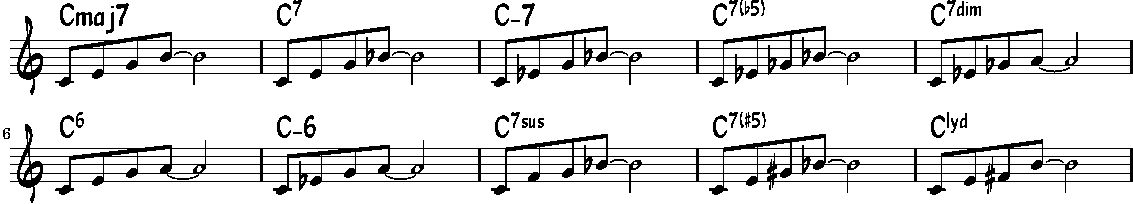
\includegraphics[width=0.98\linewidth]{arpeggios.pdf}
\end{center}
\end{document}
